Un constructor hace todas sus rampas con razón 12:1 de base a altura,
para que sean accesibles con sillas de ruedas.
Mira el diagrama de la figura \ref{fig:des_pitagoras_03a} (no dibujado a escala):
\begin{figure}[H]
    \begin{center}
        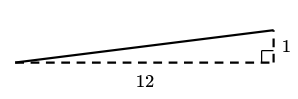
\includegraphics[width=0.4\textwidth]{../images/des_pitagoras_03a.png}
    \end{center}
    \caption{}
    \label{fig:des_pitagoras_03a}
\end{figure}
Cierta rampa necesita llegar a 0.80 metros de altura, como se muestra en la figura \ref{des_pitagoras_03b}
\begin{figure}[H]
    \begin{center}
        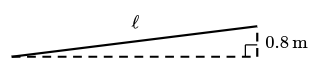
\includegraphics[width=0.4\textwidth]{../images/des_pitagoras_03b.png}
    \end{center}
    \caption{}
    \label{fig:des_pitagoras_03b}
\end{figure}
\textbf{¿Cuál es la longitud $l$ de esta rampa?}\\
\textit{Redondea tu respuesta a la centésima de metro más cercana.}